\subsection{Wasserwellen}
\enter
($ \Rightarrow $ Entstehung: Handout)
\kommentar{Handout muss hier noch nachgetragen werden.}
\begin{center}
	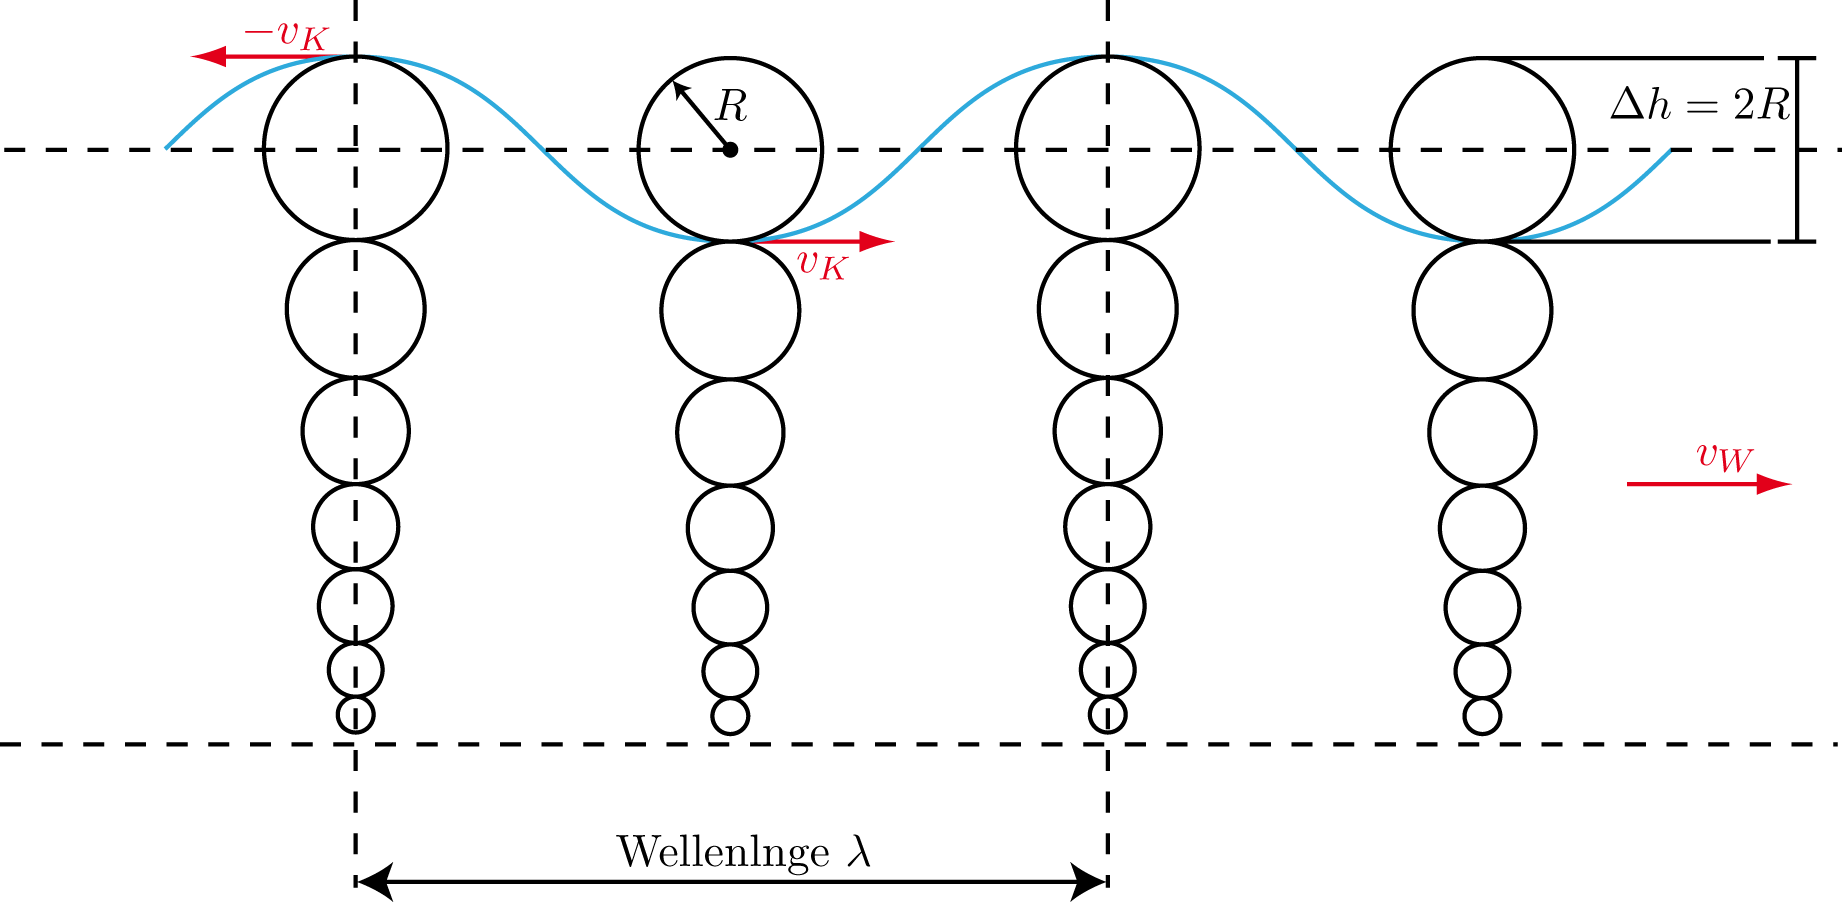
\includegraphics[width=0.7\linewidth]{skizzen/19/19B26}
\end{center}
Geschwindigkeit auf Wellenberg: $ v_{Berg} = v_W - v_K$\\
Geschwindigkeit im Wellental: $ v_{Tal} = v_{W} + v_{K} $\\
\begin{tcolorbox}[width=\textwidth*3/5,colback={White}]
Im Mittel kein Materialtransport
\end{tcolorbox}
Zunahme an kinetischer Energie vom Berg zum Tal:
$$ \Delta E^{kin} = E_{Tal}^{kin} - E_{Berg}^{kin} = \frac{1}{2} \cdot m (v_{Tal}^2 - v_{Berg}^2) 2 \cdot m \cdot v_{W} \cdot v_{K}$$
($ m $ : Masse der Wellenfront)\\
"Verlust" an potenzieller Energie:
$$ \Delta E ^{pot} = 2mgR $$
\begin{align*}
\Delta E^{pot}  = \Delta E ^{kin} \Leftarrow\\
\Rightarrow v_W = \sqrt{\frac{g\cdot\lambda_W}{2\pi}}
\end{align*}
\kommentar{"zu Hause zeigen", muss noch gemacht werden}
Schwere-wellen zeigen ausgeprägte Dispersion:
\begin{align*}
\lambda_w = \SI{10}{\meter} &\Rightarrow v_W = \SI{4}{\meter\per\second}\\
\lambda_w = \SI{1000}{\meter} &\Rightarrow v_W = \SI{40}{\meter\per\second}
\end{align*}
Für kleinere $ \lambda $ : Oberflächenspannung $ \sigma $ berücksichtigen\\
zusätzlich: Einfluss endlicher Wassertiefe berücksichtigen
\begin{center}
	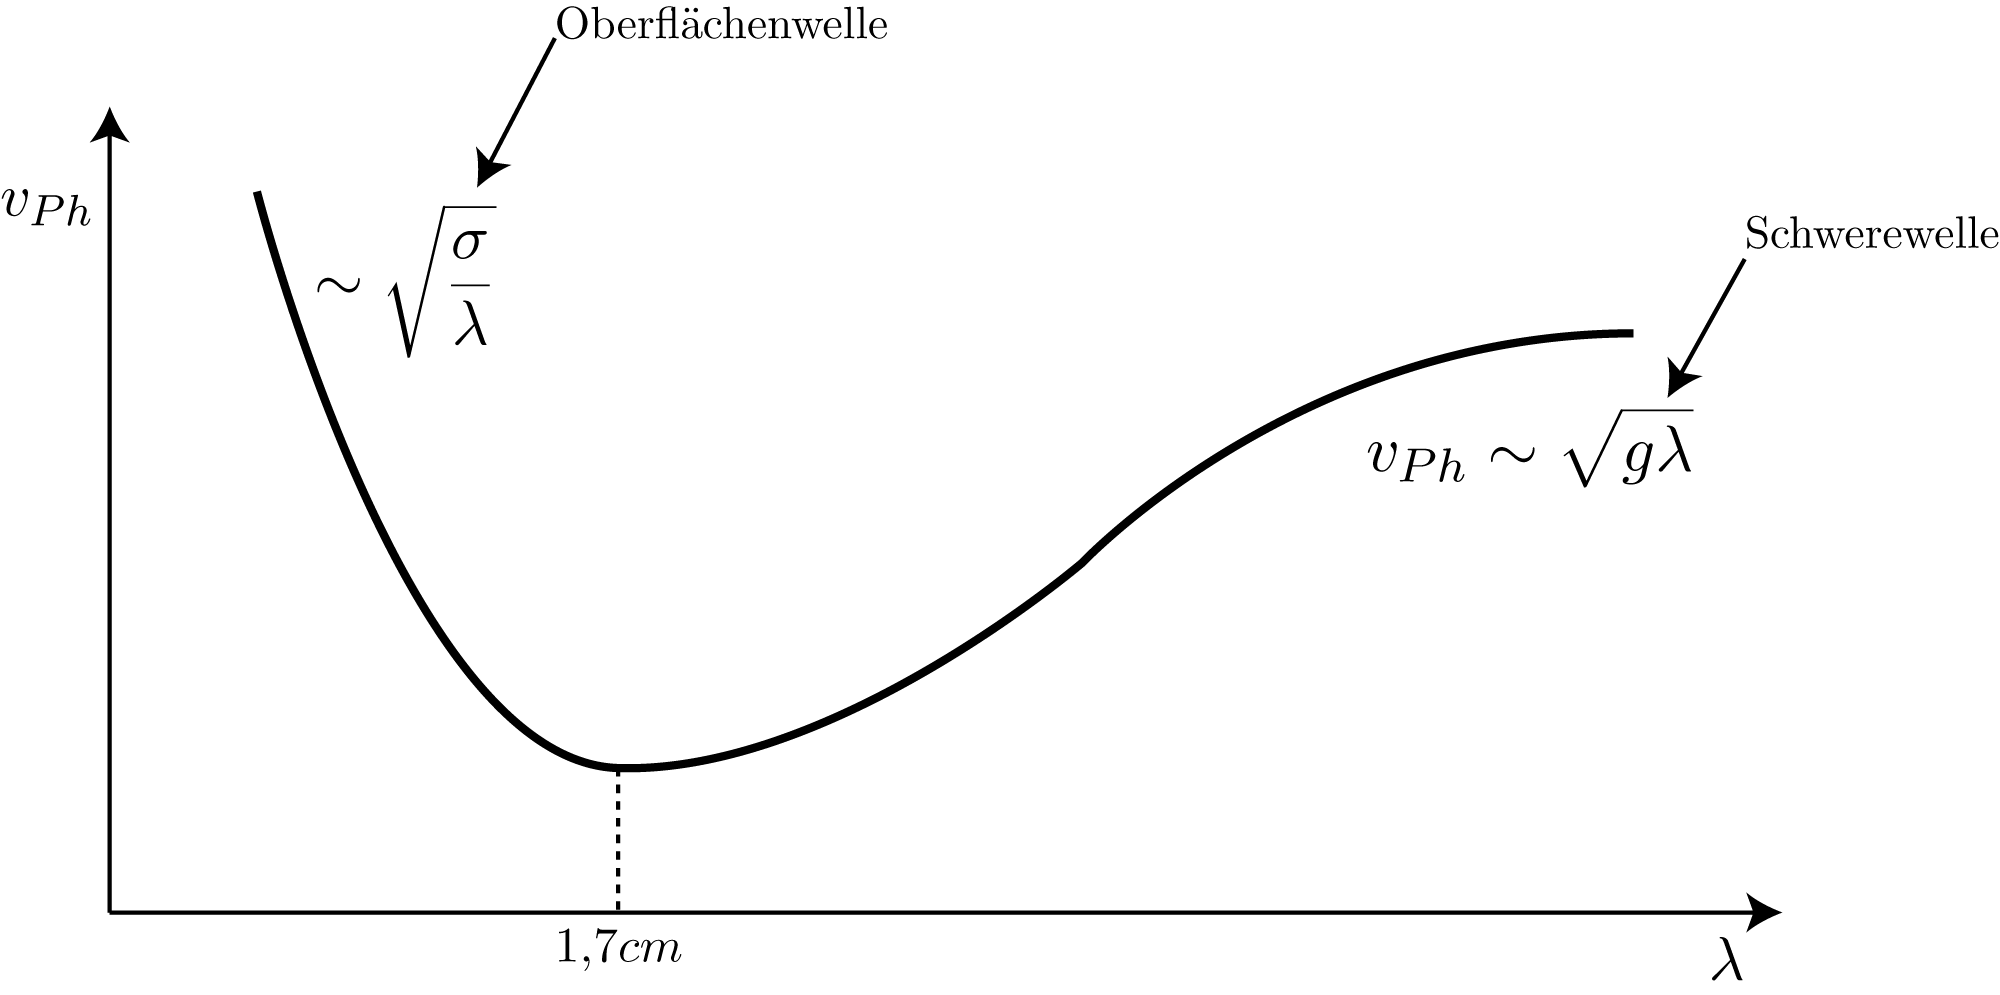
\includegraphics[width=0.7\linewidth]{skizzen/19/19B27}
\end{center}
Es gilt allgemein (Komplexe Rechnung).\\
$$ v_{Ph} = \sqrt{\frac{g\cdot\lambda_W}{2\pi}+\frac{2\pi\sigma}{\underbrace{\rho\cdot\lambda_W}_{\text{Oberfläche}}}} \cdot \overset{(A)^{1/2}}{\underset{h: \text{ Wassertiefe}}{\sqrt{\frac{1-\exp(-2\cdot K \cdot h)}{1+\exp(-2 \cdot K \cdot h)}}}}$$

\subsubsection{Seichtwasserwellen:}
ab $  n \leq \frac{\lambda_W}{4} $ muss endliche Tiefe berücksichtigt werden!\\
$$\text{(A): } \frac{1-\exp(-2Kh)}{1+\exp(-2Kh)} \overset{n<<\frac{2\pi}{K}}{\longrightarrow} \frac{1-(1-2Kh)}{1+(1-2Kh)} = \frac{2Kh}{2-2Kh} \approx Kh$$
Beschränkung auf Nicht-Oberflächenwelle:\\
$$ \rightarrow v_{Ph} = \sqrt{\frac{g\cdot\lambda_W}{2\pi}} \sqrt{\frac{2\pi}{\lambda_W}\cdot h} = \sqrt{g \cdot h} $$
Keine Dispersion für Flachwasserwelle; \underline{$ v_{Ph}  $ hängt nur von $ h $ ab!!}\\
$ \Rightarrow $ Das ist der Grund für Entstehung von Brandung und Tsünamos!\\
Experiment: Tiefwasser $ \rightarrow $ Flachwasserwelle\\
\begin{center}
	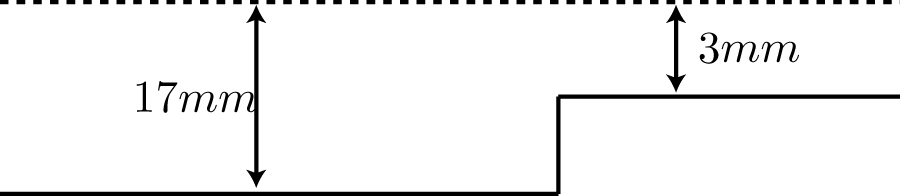
\includegraphics[width=0.5\linewidth]{skizzen/19/19B28}
\end{center}
$$ v_{Ph}  = \sqrt{g\cdot h}; \lambda_1 = \frac{v_{Ph}}{\nu} = \frac{\SI{0,41}{\meter\per\second}}{\nu}; \lambda_2 = \frac{\SI{0,17}{\meter\per\second}}{\nu} $$
$ \nu  = const.$ (Erregerfrequenz)
Entstehung von Tsünamos:\\
$ \lambda=\SI{100}{\kilo\meter} - \SI{500}{\kilo\meter} $ (z.B. durch Seebeben)\\
$ \Rightarrow $ Tsünamos sind überall Flachwasserwellen (Wellenhöhe: $ <\SI{1}{\meter} $)\\
$ v_{Ph} = \sqrt{g\cdot h} $ in Ozeanen ($ h \approx \SI{5000}{\meter} $) : $ \vDash_{Ph} =\SI{780}{\kilo\meter\per\hour} $\\
Periodendauer: $ T=\SI{7,5}{\minute} ... \SI{38}{\minute} $\\
In flachem Wasser ($ h=\SI{5}{-meter} $) reduziert sich $ v_{Ph}  $ auf ca $ 1/30 $
$$ v_{Ph}  \approx \SI{26}{\kilo\meter\per\hour}$$
$ \lambda $ reduziert sich ebenfalls auf $ 1/30 $
\begin{tcolorbox} [colback = {White}, outer arc=0mm, sharp corners]
	Da $ E_{km} $ erhalten bleibt, nimmt die Amplitude drastisch zu!!
\end{tcolorbox}